
\chapter{Power headroom estimation}

Until this point of the work, the research has been mainly focused on PSU loads forecasting. Nonetheless, as mentioned in the introductory context, the goal is to predict the power headroom defined in (\ref{eq:phdroom}). But as there are no direct measurements of power headroom that can be learnt, it is needed to derive it from the power consumption. 

Therefore, to provide a power headroom forecast, after estimating the future values of the loads' consumptions, it is needed a further step to translate that information into power headroom terms.

The following sections will propose a way to manage to achieve it and discuss other aspects of its technical applicability.

\section{Power headroom derivation as PSU utilisation complement}

As it has been exposed in section \ref{subsec:data_description:power_supply}, the power load is a measure of \emph{how many percentual power capacity it is being used at that time}. Thus, it is straightforward to claim that the percentual power headroom is its complement.

If the interest is to obtain a measurement in Watts units, the installed power capacity in the RBS, $P_{max}$, is needed to be known so that its proportion can be computed as follows.

\begin{align}\label{eq:ph_deriv}
\begin{split}
		P_{h[\%]}	&= 100 - P_{L[\%]} \\
		\text{Where }P_{h[\%]}	&: \text{Power headroom in percents} \\
		\text{and } P_{L[\%]}	&: \text{Power loads consumptions in percents}
\end{split}
\end{align}

If the interest is to obtain a measurement in Watts units, it is needed to know the installed power capacity, $P_{max}$, in the RBS so that its proportion can be computed as showed in (\ref{eq:phwatts}).

\begin{align}\label{eq:phwatts}
\begin{split}
		P_h	&= P_{max} \cdot \frac{P_{h[\%]}}{100} \\
	\text{Where } P_{max}	&: \text{Installed power capacity in Watts}
\end{split}
\end{align}

As an example, let the power load be the signal used in the forecast in chapter \ref{cha:forecasting}, and assume the installed power in the current \ac{rbs} is $12[kW]$. Then, the obtained curves are presented in Figure \ref{fig:ph_der}.

\begin{figure}[hptb]
	\centering
	\begin{subfigure}{.6\textwidth}
		\centering
		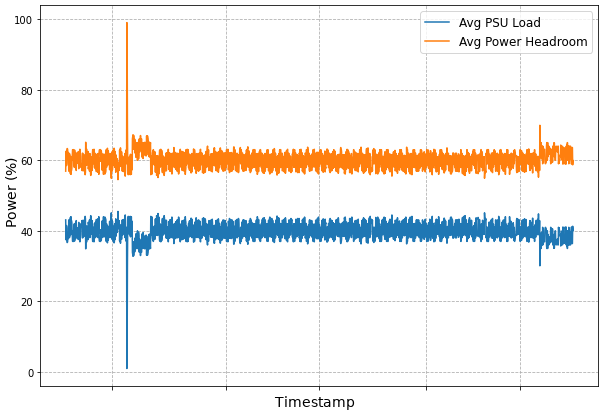
\includegraphics[width=\textwidth]{power_headroom_derivation}
		\caption{Derived power headroom in percents}
		\label{fig:ph_der_percent}
	\end{subfigure}%
	\hfill
	\begin{subfigure}{.6\textwidth}
		\centering
		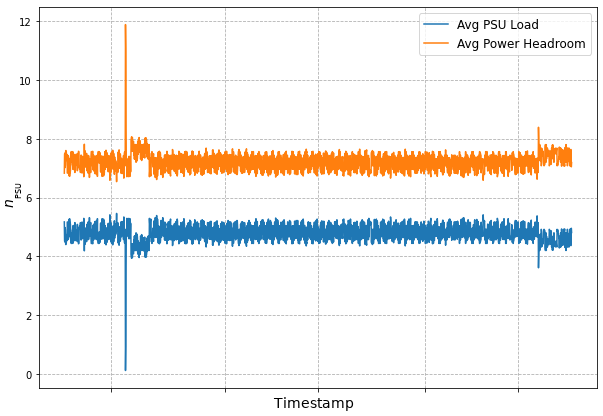
\includegraphics[width=\textwidth]{power_headroom_derivation_watts}
		\caption{Derived power headroom in Watts}
		\label{fig:ph_der_watts}
	\end{subfigure}
	\caption{Power headroom derivation from PSU Load}
	\label{fig:ph_der}
\end{figure}

\section{Criterion considerations}

In general terms, an alarm is meant to notice that something abnormal is happening in a process or, in a forecasting context, may (or will) occur in the future and support the operator response\cite{iec_alarms}.

In the current works' context, the alarm meaning can be conceived as the RBS not having enough power to manage to keep its by-design behaving.

Although it should be possible to define how likely a power overload is given the system's current state in probability terms, triggering an alarm is a binary task. The system is operating either in a \emph{"safe"}  or in an \emph{"abnormal"} region. Then crossing a boundary that separates these two regions is the trigger for the alarm. 

There are different techniques to tune an optimal trigger level. It could be done based on a system variable, or a latent variable or even a joint distribution of the two kinds\cite{izadi2009alarms}. 

Choosing the best possible boundary is considered to be out of the current work scope. Nonetheless, as an initial approach, it can be proposed to be settable by the user according to their needs and expertise. 

From this assumption and the derivations in (\ref{eq:ph_deriv}) and (\ref{eq:phwatts}) the following guidelines should be taking into consideration. 

\subsubsection*{Values interpretation}

Percentages values are not always able to fully represent the system conditions. For example, it is very different having 10\% of power headroom where the total capacity is 100 [kW] and 1 [kW] since the relative oscillations could be drastically different. Therefore, the power magnitude should be taken into consideration. 

\subsubsection*{PSUs do not partially fail}

The power capacity is not continuous. It will have discrete values as shown in Figure (\ref{fig:ph_lvls}), and also, the \acp{psu} can have different power contributions. This means that in order to set the threshold is needed to take into account the worst-case scenario, which would be \emph{"can the \ac{rbs} work if the next failure is the most power contributing \ac{psu}"}.


\begin{figure}[hptb]
	\centering
	\begin{subfigure}{.6\textwidth}
		\centering
		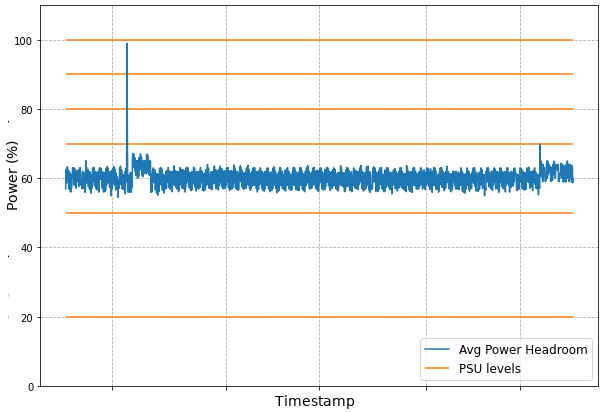
\includegraphics[width=\textwidth]{power_headroom_levels_percent}
		\caption{Power headroom and discrete availability in percents}
		\label{fig:ph_lvls_percent}
	\end{subfigure}%
	\hfill
	\begin{subfigure}{.6\textwidth}
		\centering
		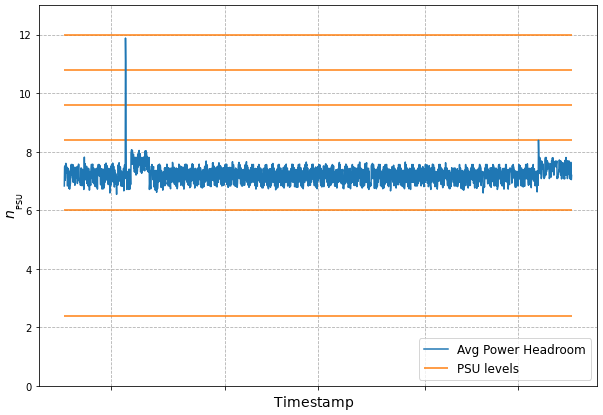
\includegraphics[width=\textwidth]{power_headroom_levels_watts}
		\caption{Power headroom and discrete availability in Watts}
		\label{fig:ph_lvls_watts}
	\end{subfigure}
	\caption{Power headroom derivation from PSU Load}
	\label{fig:ph_lvls}
\end{figure}

\pagebreak

\section{The $n$-level safety criteria}
Putting into mathematics the worst-scenario premise:

Let $N$ be the amount of PSUs installed, let $P_{PSU_1}, \ldots, P_{PSU_N}$ be the highest and the lowest power contribution from a working PSU, respectively. Then, let the $n$-level safety criteria, be the amount of worst-case \ac{psu} failures to have as operational margin:

\begin{align}
\begin{split}
	P_{max} - \sum_{i=1}^{n}{P_{PSU_i}} &> \bar{P}_{Load} + \Delta p \\
	P_{max} - \left\{\bar{P}_{Load} + \Delta p \right\} &> \sum_{i=1}^{n}{P_{PSU_i}}
\end{split}
\end{align}

But, as the power headroom is by definition the diference between the installed power capacity and the power being consumed. 

\begin{align}
	\begin{split}
		P_{h} &= P_{max} - \left\{\bar{P}_{Load} + \Delta p \right\} \\
		P_{h} &> \sum_{i=1}^{n}{P_{PSU_i}} \\
		\therefore P_{n-critical} &= \sum_{i=1}^{n}{P_{PSU_i}}
	\end{split}
\end{align}

Where $\Delta p$ is the confidence interval used when training the Prophet model.



